\section{Alit Fajar Kurniawan (1174057)}
\subsection{Penjelasan Shapefile dengan PySHP}
Shapefile merupakan sebuah format data untuk menyimpan data spasial nontopologis berbasis vektor, shapefile biasanya digunakan untuk menyimpan atau membuat data peta digital sistem informasi geografis \cite{clark2018britice}. \hfill\break
Pyshp merupakan sebuah library yang di gunakan pada python untuk dapat menjalankan shapefile. \hfill\break

\subsection{Berikut tahapan membuat shapefile dengan pyshp}
\begin{enumerate}
	\item No 1
	\lstinputlisting{src/1/1174057/alit1.py}
	\begin{figure}[H]
		
\includegraphics[width=6cm]{figures/1174057/alit1.PNG}
		\centering
		\caption{Hasil No 1}
	\end{figure}
	\item Nomor 2
	\lstinputlisting{src/1/1174057/alit2.py}
	\begin{figure}[H]
		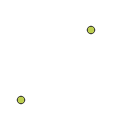
\includegraphics[width=6cm]{figures/1174057/alit2.PNG}
		\centering
		\caption{Hasil No 2}
	\end{figure}
	\item Nomor 3
	\lstinputlisting{src/1/1174057/alit3.py}
	\begin{figure}[H]
		
\includegraphics[width=6cm]{figures/1174057/alit3.PNG}
		\centering
		\caption{Hasil No 3}
	\end{figure}
	\item Nomor 4
	\lstinputlisting{src/1/1174057/alit4.py}
	\begin{figure}[H]
		
\includegraphics[width=6cm]{figures/1174057/alit4.PNG}
		\centering
		\caption{Hasil No 4}
	\end{figure}
	\item Nomor 5
	\lstinputlisting{src/1/1174057/alit5.py}
	\begin{figure}[H]
		
\includegraphics[width=6cm]{figures/1174057/alit5.PNG}
		\centering
		\caption{Hasil No 5}
	\end{figure}
	\item Nomor 6
	\lstinputlisting{src/1/1174057/alit6.py}
	\begin{figure}[H]
		
\includegraphics[width=6cm]{figures/1174057/alit6.PNG}
		\centering
		\caption{Hasil No 6}
	\end{figure}
	\item Nomor 7
	\lstinputlisting{src/1/1174057/alit7.py}
	\begin{figure}[H]
		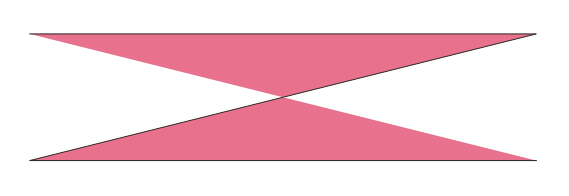
\includegraphics[width=6cm]{figures/1174057/alit7.PNG}
		\centering
		\caption{Hasil No 7}
	\end{figure}
	\item Nomor 8
	\lstinputlisting{src/1/1174057/alit8.py}
	\begin{figure}[H]
		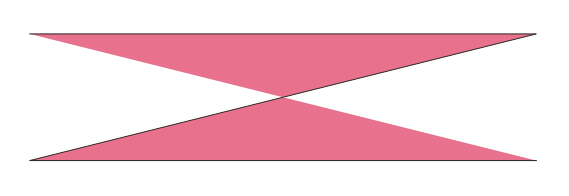
\includegraphics[width=6cm]{figures/1174057/alit8.PNG}
		\centering
		\caption{Hasil No 8}
	\end{figure}
	\item Nomor 9
	\lstinputlisting{src/1/1174057/alit9.py}
	\begin{figure}[H]
		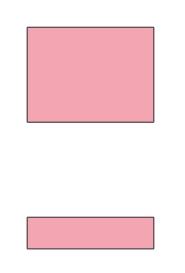
\includegraphics[width=6cm]{figures/1174057/alit9.PNG}
		\centering
		\caption{Hasil No 9}
	\end{figure}
	\item Nomor 10
	\lstinputlisting{src/1/1174057/soal10.py}
	\begin{figure}[H]
		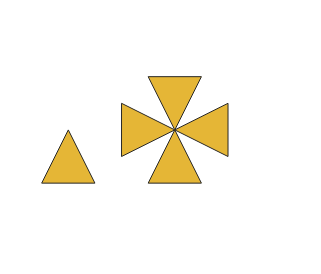
\includegraphics[width=6cm]{figures/1174057/soal10.PNG}
		\centering
		\caption{Hasil No 10, NPM saya adalah 1174057, maka hasil modulus 8 dari NPM 1174057 adalah 1, jadi membuat bidang segitaga sama sisi dan angka kedua terakhir di NPM saya adalah 5 maka saya akan membuat 5 buah segitiga sama sisi}
	\end{figure}
\end{enumerate}
\subsection{Link}
 \href{https://www.youtube.com/watch?v=vosE98eZ_Io}{Nonton Video aku di Youtube}
\subsection{Plagiarism}
\begin{figure}[H]
	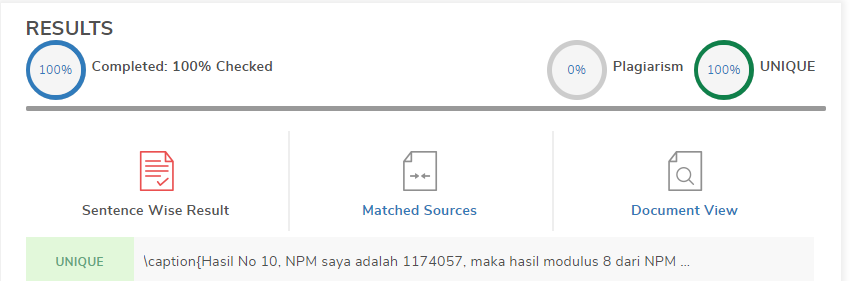
\includegraphics[width=4cm]{figures/1174057/plagiat.png}
	\centering
	\caption{Plagiarism}
\end{figure}
